%    Sidebar about panic:
% 	panic is the kernel's last resort: the impossible has happened and the
% 	kernel does not know how to proceed.  In xv6, panic does ...
\chapter{Traps, interrupts, and drivers}
\label{CH:TRAP}

When running a process, a CPU executes the normal processor loop: read an
instruction, advance the program counter, execute the instruction, repeat.  But
there are events on which control from a user program must transfer back to the
kernel instead of executing the next instruction.  These events include a device
signaling that it wants attention, a user program doing something illegal (e.g.,
references a virtual address for which there is no page table entry), or a user
program asking the kernel for a service with a system call.  There are three
main challenges in handling these events: 1) the kernel must arrange that a
processor switches from user mode to kernel mode (and back); 2) the kernel and
devices must coordinate their parallel activities; and 3) the kernel must
understand the interface of the devices.  Addressing these 3 challenges requires
detailed understanding of hardware and careful programming, and can result in
opaque kernel code.  This chapter explains how xv6 addresses these three
challenges.
%% 
\section{Systems calls, exceptions, and interrupts}
%% 
There are three cases when control must be transferred from a user program to
the kernel. First, a system call: when a user program asks for an operating
system service, as we saw at the end of the last chapter.
Second, an
\textit{exception}\index{exception}:
when a program performs an illegal action. Examples of illegal actions include
divide by zero, attempt to access memory for a page-table entry that is not
present, and so on.  Third, an
\textit{interrupt}\index{interrupt}:
when a device generates a signal to indicate that
it needs attention from the operating system.  For example, a clock chip may
generate an interrupt every 100 msec to allow the kernel to implement
time sharing.  As another example, when the disk has read a block from
disk, it generates an interrupt to alert the operating system that the
block is ready to be retrieved.

The kernel handles all interrupts, rather than processes
handling them, because in most cases only the kernel has the
required privilege and state. For example, in order to time-slice
among processes in response the clock interrupts, the kernel
must be involved, if only to force uncooperative processes to
yield the processor.

In all three cases, the operating system design must arrange for the
following to happen.  The system must save the processor's registers for future
transparent resume.  The system must be set up for execution
in the kernel.  The system must chose a place for the kernel to start
executing. The kernel must be able to retrieve information about the
event, e.g., system call arguments.  It must all be done securely; the system
must maintain isolation of user processes and the kernel.

A word on terminology: Although the official x86 term is exception,
xv6 uses the term
\textit{trap}\index{trap}, 
largely because it was the term
used by the PDP11/40 and therefore is the conventional Unix term.
Furthermore, this chapter uses the terms trap and interrupt interchangeably, but it
is important to remember that traps are caused by the current process
running on a processor (e.g., the process makes a system call and as a
result generates a trap), and interrupts are caused by devices and may
not be related to the currently running process.
For example, a disk may generate an interrupt when
it is done retrieving a block for one process, but
at the time of the interrupt some other process may be running.
This
property of interrupts makes thinking about interrupts more difficult
than thinking about traps, because interrupts happen
concurrently with other activities.
%% 
\section{X86 Interrupts}
%% 

Devices on the motherboard can generate interrupts, and xv6 must set up
the hardware to handle these interrupts.
Devices usually interrupt in order to tell the kernel that some hardware
event has occured, such as I/O completion.
Interrupts are usually optional in the sense that the kernel could
instead periodically check (or ``poll'') the device hardware to check
for new events.
Interrupts are preferable to polling if the events are relatively
rare, so that polling would waste CPU time.

Devices can generate interrupts
at any time.  There is hardware on the motherboard to signal the CPU
when a device needs attention (e.g., the user has typed a character on
the keyboard). We must program the device to generate an interrupt, and
arrange that a CPU receives the interrupt. 

Let's look at the timer device and timer interrupts.  We would like
the timer hardware to generate an interrupt, say, 100 times per
second so that the kernel can track the passage of time and so the
kernel can time-slice among multiple running processes.  The choice of
100 times per second allows for decent interactive performance while
not swamping the processor with handling interrupts.  

Like the x86 processor itself, PC motherboards have evolved, and the
way interrupts are provided has evolved too.  The early boards had a
simple programmable interrupt controler (called the PIC).
With the advent of multiprocessor PC boards, a new way of handling
interrupts was needed, because each CPU needs an interrupt controller
to handle interrupts sent to it, and there must be a method for
routing interrupts to processors.  This way consists of two parts: a
part that is in the I/O system (the IO APIC,
\lstinline{ioapic.c)}, 
and a part that is attached to each processor (the
local APIC, 
\lstinline{lapic.c).}
Xv6 is designed for a
board with multiple processors: it ignores interrupts from the PIC, and
configures the IOAPIC and local APIC.

The IO APIC has a table and the processor can program entries in the
table through memory-mapped I/O.
During initialization, xv6 programs to map interrupt 0 to IRQ 0, and
so on, but disables them all.  Specific devices enable particular
interrupts and say to which processor the interrupt should be routed.
For example, xv6 routes keyboard interrupts to processor 0
\lineref{kernel/console.c:/^consoleinit/}.
Xv6 routes disk interrupts to the highest numbered processor on the
system, as we will see later in this chapter.

The timer chip is inside the LAPIC, so that each processor can receive
timer interrupts independently. Xv6 sets it up in
\lstinline{lapicinit}\index{lapicinit@\lstinline{lapicinit}}
\lineref{kernel/lapic.c:/^lapicinit/}.
The key line is the one that programs the timer
\lineref{kernel/lapic.c:/lapicw.TIMER/}.
This line tells the LAPIC to periodically generate an interrupt at
\lstinline{IRQ_TIMER}\index{IRQ_TIMER@\lstinline{IRQ_TIMER}},
which is IRQ 0.
Line
\lineref{kernel/lapic.c:/lapicw.TPR/}
enables interrupts on a CPU's LAPIC, which will cause it to deliver
interrupts to the local processor.
%% 
\section{X86 protection and interrupt handling}
%% 

The x86 has 4 protection levels, numbered 0 (most privilege) to 3
(least privilege).  In practice, most operating systems use only 2
levels: 0 and 3, which are then called 
\textit{kernel mode}\index{kernel mode} 
and 
\textit{user mode}\index{user mode},
respectively.  The current privilege level with which the x86 executes
instructions is stored in
\texttt{\%cs}
register, in the field CPL.  On an interrupt or exception, the processor may
have to switch from user mode to kernel mode (e.g., when an interrupt arrives
while user code is running on the processor).

On the x86, interrupt handlers are defined in the interrupt descriptor
table (IDT). The IDT has 256 entries, each giving the
\texttt{\%cs}
and
\texttt{\%rip}
to be used when handling the corresponding interrupt.
% pointer to the IDT table.

When a device raises an interrupt, the x86 allows it to specify
a trap number
\textit{n}
to identify the source of the interrupt.  For example, as mentioned above, xv6
programs the timer chip to interrupt with number
\lstinline{IRQ_TIMER}
\lineref{kernel/traps.h:/IRQ_TIMER/},
which corresponds to trap
\lstinline{T_IRQ0}
\lineref{kernel/traps.h:/T_IRQ0/}.
Some trap numbers are predefined by the x86.  For example, if software
divides by zero, then the processor will use trap number
\lstinline{T_DIVIDE}\index{T_DIVIDE@\lstinline{T_DIVIDE}}
\lineref{kernel/traps.h:/T_DIVIDE/} 
to handle that exception.
The trap number is used as an index into the IDT.

On
receive an interrupt or exception, the x86 performs
the following steps:
\paragraph{\textbullet}Fetch the 
\textit{n} 'th
descriptor from the IDT,
where 
\textit{n}
is the argument of
\lstinline{int}.
\paragraph{\textbullet}Save
\texttt{\%rsp}
and
\texttt{\%ss}
in CPU-internal registers.
\paragraph{\textbullet}Sets
\texttt{\%ss}
to NULL and
loads
\texttt{\%rsp}
from a task segment descriptor.
\paragraph{\textbullet}Push saved
\texttt{\%ss}.
\paragraph{\textbullet}Push saved
\texttt{\%rsp}.
\paragraph{\textbullet}Push
\texttt{\%eflags}.
\paragraph{\textbullet}Push
\texttt{\%cs}.
\paragraph{\textbullet}Push
\texttt{\%rip}.
\paragraph{\textbullet}Clear the IF bit in
\texttt{\%eflags},
but only on an interrupt.
\paragraph{\textbullet}Set 
\texttt{\%cs}
and
\texttt{\%rip}
to the values in the IDT entry for
\lstinline{n}.

Figure~\ref{fig:intkstack} 
shows the stack after the processor receives
an interrupt or exception.
For some traps (e.g., a page fault), the processor also pushes an
error word. 

\begin{figure}[t]
\center
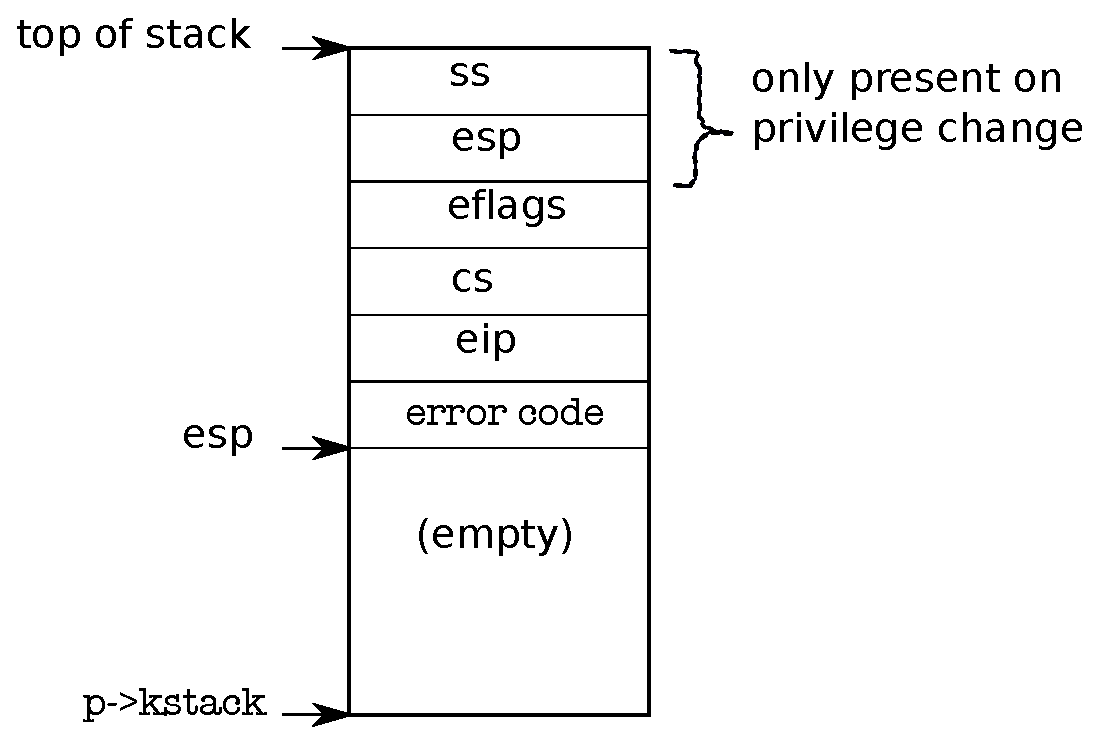
\includegraphics[scale=0.5]{fig/intkstack.eps}
\caption{Kernel stack after an interrupt or exception.}
\label{fig:intkstack}
\end{figure}

Taking interrupt or exception
is a complex step, and one might wonder whether all
these actions are necessary.
For example, is it necessary to change stacks?
The kernel shouldn't use the stack of the user process, because it may not be valid.
The user process may be malicious or
contain an error that causes the user
\texttt{\%rsp} 
to contain an address that is not part of the process's user memory.
Instead, the hardware uses the
stack specified in the task segment, which is set by the kernel.

After receiving an interrupt or exception,
the
\texttt{\%rip}
is pointing to the address specified in the descriptor table, and the
instruction at that address is the next instruction to be executed and
the first instruction of the handler for
trap number
\textit{n}.
It is job of the operating system to implement these handlers, and
below we will see what xv6 does.

An operating system can use the
\lstinline{iret}\index{iret@\lstinline{iret}}
instruction to return from an
interrupt or exception. It pops the saved values during the 
\lstinline{int}
instruction from the stack, and resumes execution at the saved
\texttt{\%rip}.

Although the description above is x86 specific, every processor has
a mechanism like this one to handle interrupts and exceptions.
%% 
\section{Code: Assembly trap handlers}
%% 

Xv6 must set up the x86 hardware to do something sensible
on encountering an
\lstinline{int}\index{int@\lstinline{int}}
instruction, which causes the processor to generate a trap.
The x86 allows for 256 different interrupts.
Interrupts 0-31 are defined for software
exceptions, like divide errors or attempts to access invalid memory addresses.
Xv6 maps the 32 hardware interrupts to the range 32-63
and uses interrupt 64 as the system call interrupt.
% pointer to the x86 exception table with vector numbers (DE, DB, ...)

\lstinline{Tvinit}
\index{tvinit}
\lineref{kernel/trap.c:/^tvinit/},
called from
\lstinline{main}\index{main@\lstinline{main}},
sets up the 256 entries in the table
\lstinline{idt}\index{idt@\lstinline{idt}}.
Interrupt
\lstinline{i}
is handled by the
code at the address in
\lstinline{vectors[i]}\index{vectors[i]@\lstinline{vectors[i]}}.
Each entry point is different, because the x86
does not provide the trap number to the interrupt handler.
Using 256 different handlers is the only way to distinguish
the 256 cases.

Xv6 programs the x86 hardware to perform a stack switch on a trap by
setting up a task segment descriptor through which the hardware loads a stack
segment selector and a new value for
\texttt{\%rsp}.
The function
\lstinline{switchuvm}\index{switchuvm@\lstinline{switchuvm}}
\lineref{kernel/vm.c:/^switchuvm/} 
stores the address of the top of the kernel stack of the user
process into the task segment descriptor.

xv6 uses a Perl script
\lineref{kernel/vectors.pl:1}
to generate the entry points that the IDT entries point to.
Each entry pushes an error code
if the processor didn't, pushes the interrupt number, and then
jumps to
\lstinline{alltraps}\index{alltraps@\lstinline{alltraps}}.

\begin{figure}[t]
\center
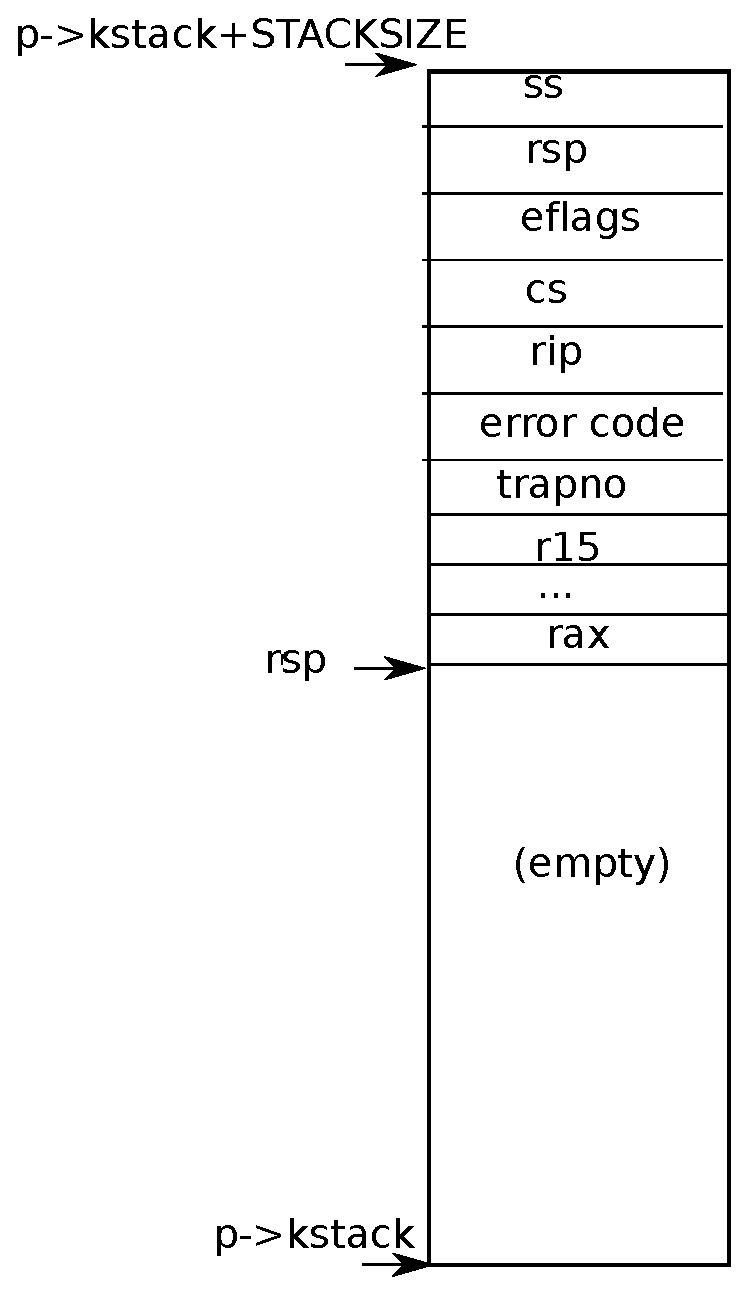
\includegraphics[scale=0.5]{fig/trapframe.eps}
\caption{The trapframe on the kernel stack}
\label{fig:trapframe}
\end{figure}

\lstinline{Alltraps}
\lineref{kernel/trapasm.S:/^alltraps/}
continues to save processor registers: it pushes
\texttt{\%r15}
through
\texttt{\%rax}.
The result of this effort is that the kernel stack now contains a
\lstinline{struct trapframe}
\lineref{kernel/x86.h:/trapframe/}
containing the processor registers at the time of the trap (see 
Figure~\ref{fig:trapframe}).
The processor pushes
\texttt{\%ss},
\texttt{\%rsp},
\texttt{\%eflags},
\texttt{\%cs}, 
and
\texttt{\%rip}.
The processor or the trap vector pushes an error number,
and 
\lstinline{alltraps}\index{alltraps@\lstinline{alltraps}} 
pushes the rest.

The trap frame contains all the information necessary
to restore the user mode processor registers
when the kernel returns to the current process,
so that the processor can continue exactly as it was when
the trap started.

Now that the user mode processor registers are saved,
\lstinline{alltraps}\index{alltraps@\lstinline{alltraps}}
can finishing setting up the processor to run kernel C code.
It passes
\texttt{\%rsp}
as a first argument to the C function
\lstinline{trap}
by moving it into
\texttt{\%rdi}
\lineref{kernel/trapasm.S:/1:mov..%rsp/},
following the C calling convention.
Thus,
\texttt{\%rdi},
the first argument,
points at the trap frame
\lstinline{alltraps}
just constructed.
Then
\lstinline{alltraps}
calls
\lstinline{trap}
\lineref{kernel/trapasm.S:/call.trap/},
which we will discus below.

After
\lstinline{trap} 
returns,
\lstinline{trapret}\index{trapret@\lstinline{trapret}}
restores the user mode registers,
popping values from the kernel stack.
Then, it discards the trap number and
the error code that trap vectors
pushed.
Finally, it returns to user
space by executing
\lstinline{iret}\index{iret@\lstinline{iret}}.
\lstinline{Iret}
pops the remaining values of the stack, loading the user stack
and program counter into
\texttt{\%rsp}
and
\texttt{\%rip},
respectively.

The discussion so far has talked about traps occurring in user mode,
but traps can also happen while the kernel is executing.
In that case the hardware does not switch stacks;
otherwise the same steps occur as in traps from user mode,
and the same xv6 trap handling code executes.
When 
\lstinline{iret}
later restores a kernel mode 
\texttt{\%cs},
the processor continues executing in kernel mode.

Xv6 calls
\lstinline{switchgs}
on system calls when switching from user to kernel mode, as we will
see below.  To make the interrupt handling and system call path
similar,
\lstinline{alltraps}
also calls
\lstinline{swapgs}
when switching from user mode, but not when
handling an interrupt in kernel mode (because it is already in kernel
mode then).
To determine whether the processor is in kernel mode,
\lstinline{alltraps}
compares the kernel code segment selector with the one saved on the stack
\lineref{kernel/trapasm.S:/cmpw..SEG_KCODE/}.
If they are the same, then there is no need to call
\lstinline{swapgs}.
Otherwise, it calls
\lstinline{swapgs}.
%% 
\section{Code: Enabling/disabling interrupts}
%% 

A processor can control if it wants to receive interrupts through the
\lstinline{IF}\index{IF@\lstinline{IF}}
flag in the
\texttt{\%eflags}
register.
The instruction
\lstinline{cli}\index{cli@\lstinline{cli}}
disables interrupts on the processor by clearing 
\lstinline{IF}, 
and
\lstinline{sti}\index{sti@\lstinline{sti}}
enables interrupts on a processor.  The bootloader disables interrupts during
booting of the main cpu
and xv6 disables interrupts when booting the other processors
\lineref{kernel/entryother.S:/cli/}.
The scheduler on each processor enables interrupts
\lineref{kernel/proc.c:/sti/}.
To control that certain code fragments are not interrupted, xv6
disables interrupts during these code fragments.  For example,
\lstinline{trapret}
above clears interrupts
\lineref{kernel/trapasm.S:/^..cli/}.
%% 
\section{Code: C trap handler}
%% 

We saw that each trap handler sets
up a trap frame and then calls the C function
\lstinline{trap}\index{trap@\lstinline{trap}}.
\lstinline{Trap}
\lineref{kernel/trap.c:/^trap\(/}
looks at the hardware trap number
\lstinline{tf->trapno}\index{tf->trapno@\lstinline{tf->trapno}}
to decide why it has been called and what needs to be done.
The timer interrupts through vector 32 (which xv6 chose to handle IRQ
0), which xv6 setup in
\lstinline{idtinit}\index{idtinit@\lstinline{idtinit}} 
\lineref{kernel/main.c:/idtinit/}.
\lstinline{Trap}
for a timer interrupt does just two things:
increment the ticks variable 
\lineref{kernel/trap.c:/ticks\+\+/}, 
and call
\lstinline{wakeup}\index{wakeup@\lstinline{wakeup}}. 
The latter, as we will see in Chapter~\ref{CH:SCHED}, may cause the
interrupt to return in a different process.
% Turns out our kernel had a subtle security bug in the way it handled traps... vb 0x1b:0x11, run movdsgs, step over breakpoints that aren't mov ax, ds, dump_cpu and single-step. dump_cpu after mov gs, then vb 0x1b:0x21 to break after sbrk returns, dump_cpu again.
% point out that we are trying to be manly with interrupts, by turning them on often in the kernel.  probably would be just fine to turn them on only when the kernel is idle.

In addition to the expected hardware
devices, a trap can be caused by a spurious interrupt, an unwanted
hardware interrupt.
% give a concrete example.
If the trap is not a system call and not a hardware device looking for
attention,
\lstinline{trap}\index{trap@\lstinline{trap}}
assumes it was caused by incorrect behavior (e.g.,
divide by zero) as part of the code that was executing before the
trap.  
If the code that caused the trap was a user program, xv6 prints
details and then sets
\lstinline{proc->killed}
to remember to clean up the user process.
We will look at how xv6 does this cleanup in Chapter~\ref{CH:SCHED}.

If it was the kernel running, there must be a kernel bug:
\lstinline{trap}
prints details about the surprise and then calls
\lstinline{panic}\index{panic@\lstinline{panic}}.
%% 
\section{Code: The first system call}
%% 

Chapter~\ref{CH:FIRST} ended with 
\lstinline{initcode.S}\index{initcode.S@\lstinline{initcode.S}}
invoking a system call.
Let's look at that again
\lineref{kernel/initcode.S:/'SYS_exec'/}.
The process pushed the arguments
for an 
\lstinline{exec}\index{exec@\lstinline{exec}}
call on the process's stack, and put the
system call number in
\texttt{\%rax}.
The system call numbers match the entries in the syscalls array,
a table of function pointers
\lineref{kernel/syscall.c:/'syscalls'/}.
We need to arrange that the 
\lstinline{syscall}
instruction switches the processor from user mode to kernel mode,
that the kernel invokes the right kernel function (i.e.,
\lstinline{sys_exec}),
and that the kernel can retrieve the arguments for
\lstinline{sys_exec}\index{sys_exec@\lstinline{sys_exec}}.
The next few subsections describe how xv6 arranges this for system
calls, and then we will discover that we can reuse the same code for
interrupts and exceptions.
%% 
\section{Code: System calls}
%% 

X86 processors for 32-bit machines handled systems calls with the same mechanism
for interrupts and exceptions, and operating systems reserved one entry in the IDT
for system calls.  X86-64 processors have a special instruction for system
calls (
\lstinline{syscall}),
which saves less state than interrupts and exceptions do, and give the operating
system more flexibility on what to save and what not to save.  This allows
operating systems to optimize code paths for specific systems calls.  For
example, for systems calls that do little work (e.g., asking what the ID is of
the current process), it is unnecessary to save and restore all the
state that interrupts and exceptions do. 

The
\lstinline{syscall}
instruction itself does less work than what the processor does on
an interrupt:
\paragraph{\textbullet}It saves
\texttt{\%eflags}
into
\texttt{\%r11}
and masks
\texttt{\%eflags}
using
a value that kernel programs into a special register reserved for this
purpose, namely
\lstinline{MSR_SFMASK}
\lineref{kernel/vm.c:/MSR_SFMASK/}.
The processor clears in
\texttt{\%eflags}
every bit corresponding to a bit that is set in the
\lstinline{MSR_SFMASK.}
\paragraph{\textbullet}It saves
\texttt{\%rip}
into
\texttt{\%rcx},
and loads
\texttt{\%rip}
with a value that the kernel programs into a special register reserved
for this purpose, namely
\lstinline{MSR_LSTAR}
\lineref{kernel/vm.c:/MSR_LSTAR/}.
Xv6 programs the address of
\lstinline{sysentry}
into this location.
\paragraph{\textbullet}It loads
\texttt{\%cs}
and
\texttt{\%ss}
selectors with values from
\lstinline{MSR_STAR}
\lineref{kernel/vm.c:/MSR_STAR/}.
xv6 programs
\lstinline{SEG_KCODE}
into
\lstinline{MSR_STAR},
which has the privilege level set to kernel mode.

Thus, after executing
\lstinline{syscall},
xv6 starts running at
\lstinline{sysentry}
\lineref{kernel/trapasm.S:/^sysentry/}
in kernel mode with interrupts disabled.
Note that the
\lstinline{syscall}
instruction doesn't consult the IDT and does not save the user's stack pointer,
unlike interrupts and exceptions. If the kernel wants
to use
\texttt{\%rsp},
it is the responsibility of the kernel to
save the value of the stack pointer before changing it.

TODO .code

Syscall allows entering into and returning from the kernel with low overhead. As
a result, a system call that can be implemented with a few assembly instructions
(e.g., return the PID of the current process) can run quickly.  The processor
executes the few steps to transfer to the kernel (saving
\texttt{\%eflags}
and
\texttt{\%rip},
and loading them with new values), then it runs the instructions for the system
call, and returns back to user space by calling
\lstinline{sysret},
which copies
\texttt{\%rcx}
into
\texttt{\%rip}
and loads
\texttt{\%eflags}
from
\texttt{\%r11}.

Xv6 doesn't optimize for performance. It always runs C code for a system call
and thus needs a stack to call into a C function.  The kernel
cannot assume that the value that a user program stored in
\texttt{\%rsp}
is save to use; the value may be an invalid address (e.g., without a mapping
in the page table).  Thus, it must save
\texttt{\%rsp}
and load it with the address of the process's kernel stack.
Where can xv6 save
\texttt{\%rsp} ?
The scratch space must be per core, because each core may
be executing a system call.

To quickly find a per-core area, the processor provides a pair of
special registers (
\lstinline{MSR_GS_BASE}\index{MSR_GS_BASE@\lstinline{MSR_GS_BASE}}
and
\lstinline{MSR_GS_KERNBASE}\index{MSR_GS_KERNBASE@\lstinline{MSR_GS_KERNBASE}})
per core.
During initialization,
each core stores a pointer to its
\lstinline{struct cpu}\index{struct cpu@\lstinline{struct cpu}}
into both registers
\lineref{kernel/vm.c:/MSR_GS_KERNBASE/}.
This struct
\lineref{kernel/proc.h:/^struct.cpu/}
records
the process currently running
on the processor (if any),
the processor's unique hardware identifier
(\lstinline{apicid}),
and some other information.
To refer to
\lstinline{MSR_GS_BASE},
the kernel must use the code segment selector
\texttt{\%gs},
which xv6 programs to contain
\lstinline{SEG_KDATA}
\lineref{kernel/vm.c:/SEG_KDATA/}.
With this setup a core can refer to
the first entry of its
\lstinline{struct cpu}
using
\lstinline{%gs}:0.
Because user code can also program
\lstinline{MSR_GS_BASE},
the processor provides a special instruction
\lstinline{swapgs},
which swaps the contents of
\lstinline{MSR_GS_BASE}
and
\lstinline{MSR_GS_KERNBASE},
causing the value of
\lstinline{MSR_GS_KERNBASE}
to be loaded into
\lstinline{MSR_GS_BASE}.
Since user code cannot program
\lstinline{MSR_GS_KERNBASE},
\lstinline{swapgs}
will cause
\lstinline{MSR_GS_BASE}
to have a valid pointer to this core's
\lstinline{struct cpu}.

Returning to
\lstinline{sysentry}
\lineref{kernel/trapasm.S:/^sysentry/},
after 
\lstinline{sysentry}
executes
\lstinline{swapps},
it saves
\texttt{\%rax}
(which contains the number of the system call)
and
\texttt{\%rsp}
(which contains the user stack pointer)
into the core's
\lstinline{struct cpu}.
The
\lstinline{struct cpu}
has reserved two fields for this purpose
\lineref{kernel/proc.h:/^struct.cpu/}.
Next,
\lstinline{sysentry}
loads the current process's kernel stack
into
\texttt{\%rsp}
\linerefs{kernel/trapasm.S:/movq...gs/,/movq...rax,..rsp/}.
Then,
\lstinline{sysentry}
restores
\texttt{\%rax},
and builds up the syscall frame
\lineref{kernel/x86.h:/^struct.sysframe/},
which we briefly saw in Chapter~\ref{CH:FIRST}. It pushes
the registers that
\lstinline{syscall}
used to store the process's instruction pointer and eflags,
along with
\texttt{\%rax}.
Next, it saves callee-saved registers and the registers
that are used to pass arguments.  It passes a pointer
to the syscall frame to the C function
\lstinline{syscall}
\lineref{kernel/syscall.c:/^syscall/}
by storing the stack pointer into the register
for the first argument.

Note that a system call saves less state than an interrupt;
\lstinline{struct sysframe}
and
\lstinline{struct trapframe}
are different.  For example, a system call doesn't save the caller-saved
registers: it is the job of the caller to save them, if it wants them to be
saved.  Interrupts can force a user process to enter the kernel at anytime, and
the process has no opportunity to save caller-saved registers or any registers
for that matter.  Thus, the hardware and xv6 must save all of a user process's
state on an interrupt so that it can be restored when returning to user space.

\lstinline{Syscall}\index{Syscall@\lstinline{Syscall}}
\lineref{kernel/syscall.c:/'^syscall'/} 
loads the system call number from the syscall frame, which
contains the saved
\texttt{\%rax},
and indexes into the system call tables.
For the first system call, 
\texttt{\%eax}
contains the value 
\lstinline{SYS_exec}\index{SYS_exec@\lstinline{SYS_exec}}
\lineref{kernel/syscall.h:/'SYS_exec'/},
and
\lstinline{syscall}
will invoke the 
\lstinline{SYS_exec} 'th 
entry of the system call table, which corresponds to invoking
\lstinline{sys_exec}.

\lstinline{Syscall}
records the return value of the system call function in
\texttt{\%eax}.
When the system call returns to user space,
\lstinline{sysexit}
\lineref{kernel/trapasm.S:/^sysexit/}
will load the values
from
\lstinline{cp->sf}\index{cp->sf@\lstinline{cp->sf}}
into the machine registers
and return to user space
using
\lstinline{sysret}.

Thus, when 
\lstinline{exec}
returns, it will return the value
that the system call handler returned
\lineref{kernel/syscall.c:/rax = syscalls/}.
System calls conventionally return negative numbers to indicate
errors, positive numbers for success.
If the system call number is invalid,
\lstinline{syscall}\index{syscall@\lstinline{syscall}}
prints an error and returns \-1.

\lstinline{sysexit}
disables interrupts
while restoring machine registers and the user stack to
ensure that an interrupt doesn't run on a user stack.  After
\lstinline{mov (%rsp),%rsp},
the user stack is in
\texttt{\%rsp}
but the processor is still in kernel mode.
Thus, if an interrupt arrives right after this
\lstinline{mov}
instruction,
the processor will not switch to a kernel stack (because it is still in kernel
mode) and will attempt to the user stack, which may not be valid.
By disabling interrupts,
\lstinline{sysexit}
ensures that this situation can never happen.
%% 
\section{Code: System call arguments}
%% 

Later chapters will examine the implementation of
particular system calls.
This chapter is concerned with the mechanisms for system calls.
There is one bit of mechanism left: finding the system call arguments.
The helper functions
\lstinline{argint},
\lstinline{argaddr},
\lstinline{argptr},
\lstinline{argstr},
and
\lstinline{argfd}
retrieve the 
\textit{n} 'th 
system call
argument, as either an integer, pointer, a string, or a file descriptor.
\lstinline{argint}\index{argint@\lstinline{argint}}
and
\lstinline{argaddr}\index{argaddr@\lstinline{argaddr}}
use the function
\lstinline{fetcharg}
to locate the
\textit{n}'th 
argument. The C calling conventions specify that argument 0 is passed
through
\texttt{\%rdi},
argument 1 through
\texttt{\%rsi},
argument 2 through
\texttt{\%rdx},
argument 3 through
\texttt{\%r10},
argument 4 through
\texttt{\%r8},
and argument 5 through
\texttt{\%r9}.

\lstinline{argint} 
calls 
\lstinline{fetchint}\index{fetchint@\lstinline{fetchint}}
to read the value at that address from user memory and write it to
\lstinline{*ip}.  
\lstinline{fetchint} 
can simply cast the address to a pointer, because the user and the
kernel share the same page table, but the kernel must verify that the
pointer lies within the user part of the address
space.
The kernel has set up the page-table hardware to make sure
that the process cannot access memory outside its local private memory:
if a user program tries to read or write memory at an address of
\lstinline{p->sz}\index{p->sz@\lstinline{p->sz}} 
or above, the processor will cause a segmentation trap, and trap will
kill the process, as we saw above.
The kernel, however,
can derefence any address that the user might have passed, so it must check explicitly that the address is below
\lstinline{p->sz}.

\lstinline{fetchaddr}\index{fetchaddr@\lstinline{fetchaddr}},
is like
\lstinline{fetchint},
but retrieves 64-bit value instead of a 32-bit int.

\lstinline{argptr}\index{argptr@\lstinline{argptr}}
fetches the
\textit{n} th 
system call argument and checks that this argument is a valid
user-space pointer.

\lstinline{argstr}\index{argstr@\lstinline{argstr}} 
interprets the
\textit{n} th 
argument as a pointer.  It ensures that the pointer points at a
NUL-terminated string and that the complete string is located below
the end of the user part of the address space.

Finally,
\lstinline{argfd}\index{argfd@\lstinline{argfd}}
\lineref{kernel/sysfile.c:/^argfd/}
uses
\lstinline{argint}
to retrieve a file descriptor number, checks if it is valid
file descriptor, and returns the corresponding
\lstinline{struct}
\lstinline{file}.

The system call implementations (for example, sysproc.c and sysfile.c)
are typically wrappers: they decode the arguments using 
\lstinline{argint},
\lstinline{argaddr},
\lstinline{argptr}, 
and 
\lstinline{argstr}
and then call the real implementations.
In chapter~\ref{CH:MEM},
\lstinline{sys_exec}
uses these functions to get at its arguments.


%% 
\section{Drivers}
%% 
A
\textit{driver}\index{driver}
is the code in an operating system that manages a particular device:
it tells the device hardware to perform operations,
configures the device to generate interrupts when done,
and handles the resulting interrupts.
Driver code can be tricky to write
because a driver executes concurrently with the device that it manages.  In
addition, the driver must understand the device's interface (e.g., which I/O
ports do what), and that interface can be complex and poorly documented.

The disk driver provides a good example.  The disk driver copies data
from and back to the disk.  Disk hardware traditionally presents the data on the
disk as a numbered sequence of 512-byte 
\textit{blocks} 
\index{block}
(also called 
\textit{sectors}): 
\index{sector}
sector 0 is the first 512 bytes, sector 1 is the next, and so on. The block size
that an operating system uses for its file system maybe different than the
sector size that a disk uses, but typically the block size is a multiple of the
sector size.  Xv6's block size is identical to the disk's sector size.  To
represent a block xv6 has a structure
\lstinline{struct buf}
\lineref{kernel/buf.h:/^struct.buf/}.
The
data stored in this structure is often out of sync with the disk: it might have
not yet been read in from disk (the disk is working on it but hasn't returned
the sector's content yet), or it might have been updated but not yet written
out.  The driver must ensure that the rest of xv6 doesn't get confused when the
structure is out of sync with the disk.
%% 
%%  -------------------------------------------
%% 
\section{Code: Disk driver}

The IDE device provides access to disks connected to the
PC standard IDE controller.
IDE is now falling out of fashion in favor of SCSI and SATA,
but the interface is simple and lets us concentrate on the
overall structure of a driver instead of the details of a
particular piece of hardware.

Xv6 represent file system blocks using
\lstinline{struct buf}\index{struct buf@\lstinline{struct buf}}
\lineref{kernel/buf.h:/^struct.buf/}.
\lstinline{BSIZE}
\lineref{kernel/fs.h:/BSIZE/}
is identical to the IDE's sector size and thus
each buffer represents the contents of one sector on a particular
disk device.  The
\lstinline{dev}
and
\lstinline{sector}
fields give the device and sector
number and the
\lstinline{data}
field is an in-memory copy of the disk sector.
Although the xv6 file system chooses
\lstinline{BSIZE}
to be identical to the IDE's sector size, the driver can handle
a
\lstinline{BSIZE}
that is a multiple of the sector size. Operating systems often use
bigger blocks than 512 bytes to obtain higher disk throughput.

The
\lstinline{flags}
track the relationship between memory and disk:
the
\lstinline{B_VALID}\index{B_VALID@\lstinline{B_VALID}}
flag means that
\lstinline{data}
has been read in, and
the 
\lstinline{B_DIRTY}\index{B_DIRTY@\lstinline{B_DIRTY}} 
flag means that
\lstinline{data}
needs to be written out.

The kernel initializes the disk driver at boot time by calling
\lstinline{ideinit}\index{ideinit@\lstinline{ideinit}}
\lineref{kernel/ide.c:/^ideinit/}
from
\lstinline{main}\index{main@\lstinline{main}}
\lineref{kernel/main.c:/ideinit/}.
\lstinline{Ideinit}
calls
\lstinline{ioapicenable}\index{ioapicenable@\lstinline{ioapicenable}}
to enable the
\lstinline{IDE_IRQ}\index{IDE_IRQ@\lstinline{IDE_IRQ}}
interrupt
\lineref{kernel/ide.c:/ioapicenable/}.
The call to
\lstinline{ioapicenable}
enables the interrupt only on the last CPU
\lstinline{ncpu-1}): (
on a two-processor system, CPU 1 handles disk interrupts.

Next,
\lstinline{ideinit}\index{ideinit@\lstinline{ideinit}}
probes the disk hardware.
It begins by calling
\lstinline{idewait}\index{idewait@\lstinline{idewait}}
\lineref{kernel/ide.c:/idewait.0/}
to wait for the disk to
be able to accept commands.
A PC motherboard presents the status bits of the disk hardware on I/O port
\texttt{0x1f7}.
\lstinline{Idewait}
\lineref{kernel/ide.c:/^idewait/}
polls the status bits until the busy bit
(\lstinline{IDE_BSY}\index{IDE_BSY@\lstinline{IDE_BSY}})
is clear and the ready bit
(\lstinline{IDE_DRDY}\index{IDE_DRDY@\lstinline{IDE_DRDY}})
is set.

Now that the disk controller is ready,
\lstinline{ideinit}
can check how many disks
are present.
It assumes that disk 0 is present,
because the boot loader and the kernel
were both loaded from disk 0,
but it must check for disk 1.
It writes to I/O port
\texttt{0x1f6}
to select disk 1
and then waits a while for the status bit to show
that the disk is ready
\linerefs{kernel/ide.c:/Check.if.disk.1/,/^..}/}.
If not, 
\lstinline{ideinit}
assumes the disk is absent.

After
\lstinline{ideinit},
the disk is not used again until the buffer cache calls
\lstinline{iderw}\index{iderw@\lstinline{iderw}},
which updates a locked buffer
as indicated by the flags.
If
\lstinline{B_DIRTY}\index{B_DIRTY@\lstinline{B_DIRTY}}
is set,
\lstinline{iderw}
writes the buffer
to the disk; if
\lstinline{B_VALID}\index{B_VALID@\lstinline{B_VALID}}
is not set,
\lstinline{iderw}\index{iderw@\lstinline{iderw}}
reads the buffer from the disk.

Disk accesses typically take milliseconds,
a long time for a processor.
The boot loader
issues disk read commands and reads the status
bits repeatedly until the data is ready (see Appendix~\ref{APP:BOOT}).
This 
\textit{polling}\index{polling} 
or 
\textit{busy waiting}\index{busy waiting}
is fine in a boot loader, which has nothing better to do.
In an operating system, however, it is more efficient to
let another process run on the CPU and arrange to receive
an interrupt when the disk operation has completed.
\lstinline{Iderw}
takes this latter approach,
keeping the list of pending disk requests in a queue
and using interrupts to find out when each request has finished.
Although
\lstinline{iderw}
maintains a queue of requests,
the simple IDE disk controller can only handle
one operation at a time.
The disk driver maintains the invariant that it has sent
the buffer at the front of the queue to the disk hardware;
the others are simply waiting their turn.

\lstinline{Iderw}
\lineref{kernel/ide.c:/^iderw/}
adds the buffer
\lstinline{b}
to the end of the queue
\linerefs{kernel/ide.c:/Append/,/pp.=.b/}.
If the buffer is at the front of the queue,
\lstinline{iderw}\index{iderw@\lstinline{iderw}}
must send it to the disk hardware
by calling
\lstinline{idestart}\index{idestart@\lstinline{idestart}}
\lineref{kernel/ide.c:/Start.disk/,/idestart/};
otherwise the buffer will be started once
the buffers ahead of it are taken care of.

\lstinline{Idestart}
\lineref{kernel/ide.c:/^idestart/}
issues either a read or a write for the buffer's device and sector,
according to the flags.
If the operation is a write,
\lstinline{idestart}
must supply the data now
\lineref{kernel/ide.c:/outsl/}.
\lstinline{idestart}
moves the data to a buffer in the disk controller
using the
\lstinline{outsl}
instruction; 
using CPU instructions to move data to/from device hardware
is called programmed I/O.
Eventually the disk hardware will raise an
interrupt to signal that the data has been written to disk.
If the operation is a read, the interrupt will signal that the
data is ready, and the handler will read it.
Note that
\lstinline{idestart}\index{idestart@\lstinline{idestart}}
has detailed knowledge about the IDE device, and writes the right values at the
right ports.  If any of these 
\lstinline{outb}
statements is wrong, the IDE will do something differently than what we want.
Getting these details right is one reason why writing device drivers is
challenging.

Having added the request to the queue and started it if necessary,
\lstinline{iderw}
must wait for the result.  As discussed above,
polling does not make efficient use of the CPU.
Instead,
\lstinline{iderw}\index{iderw@\lstinline{iderw}}
yields the CPU for other processes by sleeping,
waiting for the interrupt handler to 
record in the buffer's flags that the operation is done
\linerefs{kernel/ide.c:/while.*VALID/,/sleep/}.
While this process is sleeping,
xv6 will schedule other processes to keep the CPU busy.

Eventually, the disk will finish its operation and trigger an interrupt.
\lstinline{trap}\index{trap@\lstinline{trap}}
will call
\lstinline{ideintr}\index{ideintr@\lstinline{ideintr}}
to handle it
\lineref{kernel/trap.c:/ideintr/}.
\lstinline{Ideintr}
\lineref{kernel/ide.c:/^ideintr/}
consults the first buffer in the queue to find
out which operation was happening.
If the buffer was being read and the disk controller has data waiting,
\lstinline{ideintr}
reads the data from a buffer in the disk controller
into memory with
\lstinline{insl}\index{insl@\lstinline{insl}}
\linerefs{kernel/ide.c:/Read.data/,/insl/}.
Now the buffer is ready:
\lstinline{ideintr}
sets 
\lstinline{B_VALID}\index{B_VALID@\lstinline{B_VALID}},
clears
\lstinline{B_DIRTY}\index{B_DIRTY@\lstinline{B_DIRTY}},
and wakes up any process sleeping on the buffer
\linerefs{kernel/ide.c:/Wake.process/,/wakeup/}.
Finally,
\lstinline{ideintr}
must pass the next waiting buffer to the disk
\linerefs{kernel/ide.c:/Start.disk/,/idestart/}.
%% 
\section{Real world}
%% 
Supporting all the devices on a PC motherboard in its full glory is much work,
because there are many devices, the devices have many features, and the protocol
between device and driver can be complex.  In many operating systems, the
drivers together account for more code in the operating system than the core
kernel.

Actual device drivers are far more complex than the disk driver in this chapter,
but the basic ideas are the same:
typically devices are slower than CPU, so the hardware uses
interrupts to notify the operating system of status changes.
Modern disk controllers typically
accept a 
\textit{batch}\index{batch} 
of disk requests at a time and even reorder
them to make most efficient use of the disk arm.
When disks were simpler, operating systems often reordered the
request queue themselves.

Many operating systems have drivers for solid-state disks because they provide
much faster access to data.  But, although a solid-state disk works very differently
from a traditional mechanical disk, both devices provide block-based interfaces
and reading/writing blocks on a solid-state disk is still more expensive than
reading/writing RAM.

Other hardware is surprisingly similar to disks: network device buffers
hold packets, audio device buffers hold sound samples, graphics card
buffers hold video data and command sequences.
High-bandwidth devices—disks, graphics cards, and network cards—often use
direct memory access (DMA) instead of programmed I/O
TODO .opcode insl , (

TODO .opcode outsl ).

DMA allows the device direct access to physical memory.
The driver gives the device the physical address of the buffer's data and
the device copies directly to or from main memory,
interrupting once the copy is complete.
DMA is faster and more efficient than programmed I/O
and is less taxing for the CPU's memory caches.

Some drivers dynamically switch between polling and interrupts, because using
interrupts can be expensive, but using polling can introduce delay until the
driver processes an event.  For example, a network driver that receives a
burst of packets may switch from interrupts to polling since it knows that more
packets must be processed and it is less expensive to process them using polling.
Once no more packets need to be processed, the driver may switch back to
interrupts, so that it will be alerted immediately when a new packet arrives.

The IDE driver routes interrupts statically to a particular processor.  Some
drivers configure the IO APIC
to route interrupts to multiple processors to spread out
the work of processing packets.
For example, a network driver might arrange to deliver interrupts
for packets of one network connection to the processor that is managing that
connection, while interrupts for packets of another connection are delivered to
another processor.  This routing can get quite sophisticated; for example, if
some network connections are short lived while others are long lived and the
operating system wants to keep all processors busy to achieve high throughput.

If a program reads a file, the data for that file is copied twice.  First, it
is copied from the disk to kernel memory by the driver, and then later it is
copied from kernel space to user space by the 
\lstinline{read}
system call.  If the program then sends the data over the network, 
the data is copied twice more: from user space to kernel space and from
kernel space to the network device.  To support applications for which 
efficiency is important (e.g., serving popular images on the Web), operating systems
use special code paths to avoid copies.  As one example,
in real-world operating systems, 
buffers typically match the hardware page size, so that
read-only copies can be mapped into a process's address space
using the paging hardware, without any copying.
%% 
\section{Exercises}
%% 

1. Set a breakpoint in
\lstinline{trap}
to catch the first timer interrupt. What values are on the stack at this
point?  Explain the output of x/37x
\texttt{\%rsp}
at that breakpoint with each value
labeled as to what it is (e.g., saved
\texttt{\%ebp}
for trap, trapframe.rip, scratch space, etc.).

2.  Add a new system call to get the current UTC time and return it to the user
program. You may want to use the helper function,
\lstinline{cmostime}
\lineref{lapic.c:/cmostime/},
to read the real time clock. The file date.h contains the definition
of the
\lstinline{struct rtcdate}
\lineref{date.h:/rtcdate/},
which you will provide as an argument to
\lstinline{cmostime}
as a pointer.

3. Write a driver for a disk that supports the SATA standard (search for SATA on
the Web). Unlike IDE, SATA isn't obsolete.  Use SATA's tagged command queuing to
issue many commands to the disk so that the disk internally can reorder commands
to obtain high performance.

4. Add simple driver for an Ethernet card.
